\chapter{Arhitectura aplicaţiei}

Proiectată privind către viitor, aplicaţia noastră oferă posibilitatea 
extinderii pe viitor în numeroase direcţii de dezvoltare. Am construit o 
platformă solidă pe baza căreia se poate dezvolta o aplicaţie CAD de un nivel 
comparabil cu a altor aplicaţii de acest tip.

Vom orienta prezentarea noastră în două direcţii. Întîi ne vom concentra asupra 
modelului de lucru. El reprezintă inima proiectului, un concept care uneşte în 
el toate capacităţile acestui proiect. Apoi vom trece la descrierea interfeţei 
cu utilizatorul, a cărei concepţie în sine prezintă o considerăm remarcabilă şi 
reprezintă o bază pentru dezvoltări ulterioare.

\section{Modelul de lucru}

\begin{definition}
\label{define:model}
Numim \textbf{Model de lucru} reprezentarea într-o colecţie de obiecte Java a 
unei structuri arhitecturale ce poate fi modelată cu ajutorul acestui 
proiect.
\end{definition}

Modelul de lucru este o reprezentare a unei structuri pe care proiectantul 
doreşte să o reprezinte cu această unealtă într-o formă pe care programul o 
poate recunoaşte şi o poate reface cît mai fidel cu modelul real imaginat de 
proiectant.

\begin{definition}
\label{define:primitive}
Numim \textbf{Primitivă} unitatea structurală şi funcţională a Modelului de 
lucru. O primitivă poate fi o colecţie de alte primitive. De asemenea, o 
primitivă este un element ce poate fi materializat atît la nivel logic cît şi 
într-o reprezentare grafică.
\end{definition}

Primitivele sunt analogiile entităţilor logice în care un model real poate fi 
divizat pentru a-l reprezenta structurat. În seria de primitive ce pot apare în 
modelul logic pot exista primitive care nu au un analog imediat în lumea reală.

\begin{statement}
Modelul logic în totalitatea lui este o Primitivă.
\end{statement}

Plecînd de la aceste două noţiuni, vom încerca să prezentăm întreaga structură 
a Modelului de lucru şi modul în care acesta interacţionează cu aplicaţia în 
sine.

În esenţă, o primitivă este orice poate fi desenat. De aceea, la rîndul său 
modelul este o primitivă. Introducem două direcţii în care modelul poate fi 
reprezentat.

\begin{definition}
Numim \textbf{Reprezentare Reală} o materializare strictă în comenzi 
Java/OpenGL a unei reprezentări schematice tridimensionale a unei Primitive, 
realizată cu scopul formării unei imaginii asupra rezultatului final al 
construcţiei fizice a entităţii logice din spatele acelei 
primitive.
\end{definition} Modelul tridimensional este deci cea mai apropiată 
formă de realitate pe care acest proiect o va reda pentru utilizatorii săi.

\begin{definition}
\label{define:editorRender}
Numim \textbf{Reprezentare Editabilă} o materializare strictă în comenzi 
Java/OpenGL a unei reprezentări schematice bidimensionale a unei Primitive, 
realizată cu scopul identificării vizuale a primitivelor şi accesării facilă 
prin intermediul unui editor a proprietăţilor primitivelor.
\end{definition}

Reprezentarea Editabilă este apropiată ca raţiune figurilor din desenul tehnic, 
şi de aceea identitatea lor vizuală este la rîndul ei asemănătoare acelor 
figuri. Alegerea acestor noţiuni este în strictă corelaţie cu detaliile de 
implementare ale aplicaţiei, care le vom detalia în următorul capitol. Pentru a 
ne face o idee despre cum aceste două reprezentări se potrivesc peste model, 
vom spune că reprezentarea modelului de lucru este juxtapunerea tuturor 
reprezentărilor celorlalte primitive existente în model, în ambele 
reprezentări. Desigur, asta implică că modelul în sine nu este decît un simplu 
container logic pentru toate celelalte componente ale aplicaţiei.

\subsection{Tipuri de primitive}

Alegerea setului de primitive de care va dispune această aplicaţie a fost o 
sarcină dificilă. Timpul de implementare este în directă corelaţie cu volumul 
de primitive care trebuiesc implementate.

Vom lăsa ca un exerciţiu viitor adăugarea de noi primitive care ar fi de un 
real ajutor utilizatorului acestei aplicaţii. Setul ales este considerat de 
autor ca fiind suficient pentru a oferi un set de funcţionalităţi de bază 
utilizabile pentru această aplicaţie şi destul de variate pentru a scoate în 
evidenţă potenţialul de creştere al acestui proiect.

\subsubsection{Ziduri şi Colţuri de Ziduri}

Elementele constructive esenţiale ale unei structuri sunt zidurile. Ele 
delimitează forma şi suprafaţa construcţiei, avînd un impact crucial asupra 
preţului de construcţie şi facilităţile ce vor putea fi oferite de acea 
construcţie.

Colţurile sunt un tip de primitivă indirect disponibilă proiectantului. Unirea 
capetelor a două ziduri se poate face printr-un colţ, care introduce de fapt o 
legătură permanentă între marginile acelor două ziduri. Constrîngerea este una 
punctuală, zidurile putînd avea orice orientare în cadrul modelului atîta timp 
cît sunt conectate la un colţ. Colţurile pot fi privite ca nişte puncte într-un 
plan.

Orice zid este conectat la două colţuri, \textbf{Colţul de Start} şi 
\textbf{Colţul de Stop}. Astfel poziţionat, lungimea şi orientarea unui zid 
este dictată de poziţia celor două colţuri. Astfel, un zid poate fi privit ca 
un segment ce leagă oricare două puncte (colţuri) dintr-un plan.

\subsubsection{Caracteristici de Ziduri}

\begin{definition}
\label{define:feature}
Numim \textbf{Caracteristică a unui Zid} orice Primitivă ce este asociată în 
mod direct cu un zid.
\end{definition}

Toate Caractersticile sunt constrînse poziţional în lungimea zidului. Ele 
adaugă elemente suplimentare modelului care sunt strict legate în realitate de 
existenţa unui zid. Exemple tipice de caracterstici ce elucidează şi mai bine 
ce reprezintă o caracteristică ar fi:

\begin{itemize}
  \item Fereastră
  \item Uşă
  \item Deschidere -- orice 
trecere completă prin volumul unui zid (o intrare fără
  uşă, sau deschiderea 
unei ferestre fără o fereastră montată în ea)
  \item Cavitate -- orice intrare 
parţială în volumul unui zid, ca un raft
  interior într-un perete fals.
\item Ingroşăre -- orice adăugare la volumul unui zid, o îngroşare într-o 
anumită zonă, ce poate servi, prin analogie, ca un raft exterior într-un 
perete.
\end{itemize}
  
\subsubsection{Decoraţiuni}
  
\begin{definition}
\textbf{Decoraţiunile} sunt Primitive care nu au legătură strictă cu structura 
construită, însă oferă un plus de realism şi poate sugera viitoarea destinaţie 
a diferitelor spaţii din model.
\end{definition}
  
\begin{itemize}
  \item Canapea
  \item Masă
  \item Toaletă
  \item Chiuvetă de baie
  \item Vană
  \item Chiuvetă de bucătărie
  \item Aragaz
  \item Frigider
  \item Masă de bucătărie
\end{itemize}

Dintre aceste Decoraţiuni, unele dintre ele vor fi implementate ca şi 
Caracterstici, datorită constrîngerii lor reale de a apărea pe un zid. Dintre 
cele menţionate mai sus, dăm exemplu chiuveta care întotdeauna apare în 
vecinătatea unui perete.

În Figura \ref{figure:model-arh} vom sumariza cele prezentate mai sus printr-o 
diagramă cu toate componentele modelului de lucru.

\begin{figure}[htp]
\begin{center} 
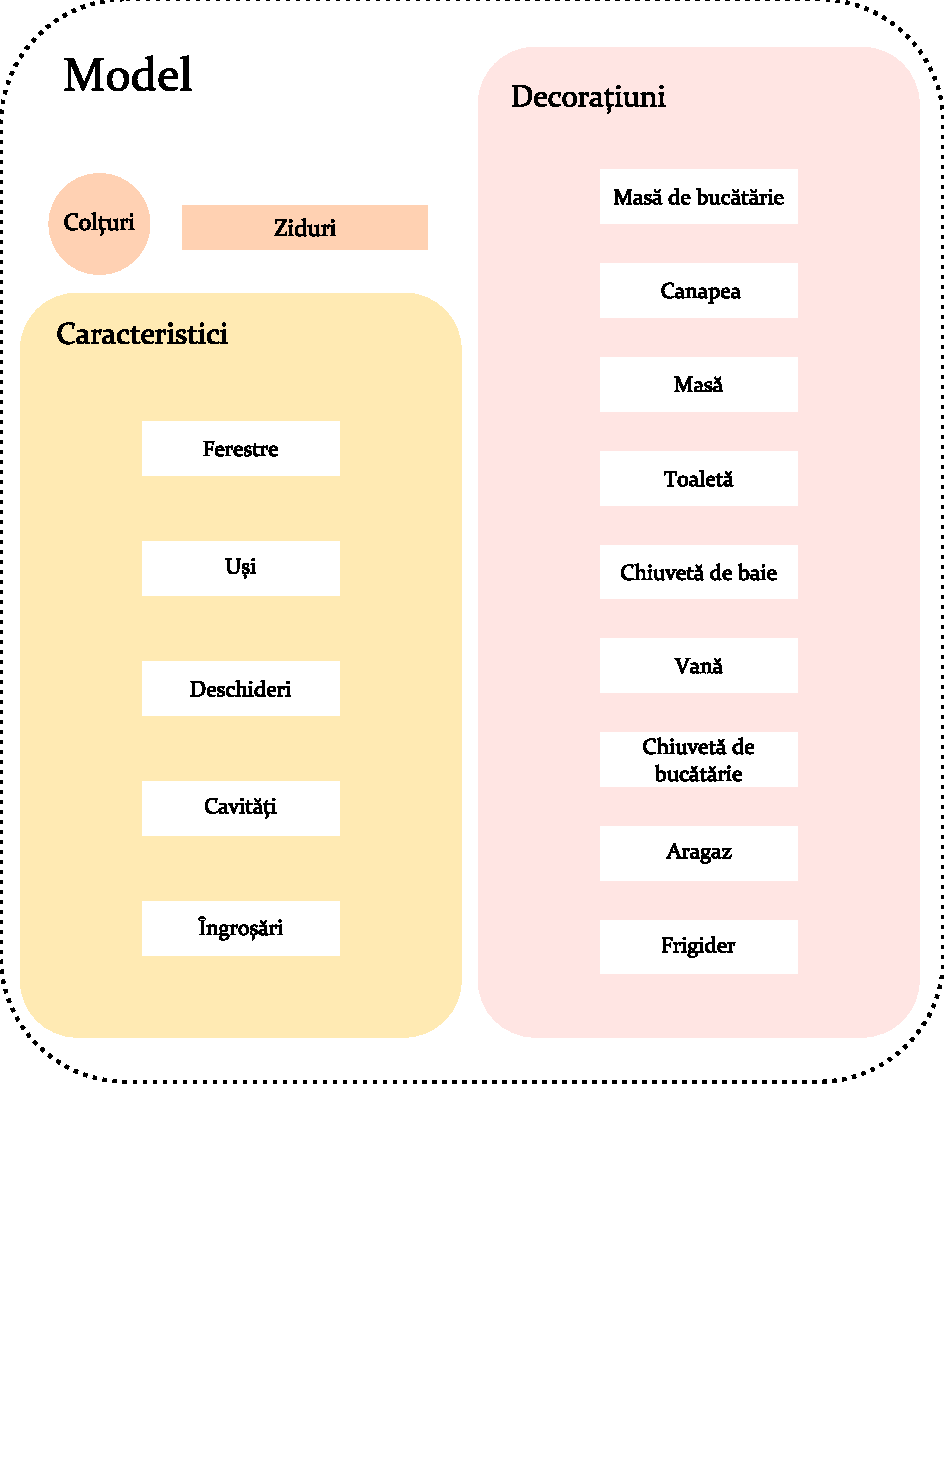
\includegraphics[width=\textwidth]{figures/drawing.pdf}
  \caption{Arhitectura 
Modelului de Lucru}
  \label{figure:model-arh}
\end{center}
\end{figure}


\section{Editorul OpenGL}

Înainte de a fi un editor pentru Modelul de Lucru (Definiţia 
\ref{define:model}), editorul OpenGL dezvoltat de noi este un punct de plecare 
foarte bun pentru orice editor care necesită folosirea facilităţilor OpenGL. 
Vom încerca să descriem succint arhitectura editorului, evidenţiind 
caracteristicile generice cît şi particularizările de suprafaţă care au fost 
necesare pentru integrarea cu funcţionarea dorită.

Editorul este în principiu o suprafaţă de desenare OpenGL cu aspect 
bidimensional ce poate interacţiona cu utilizatorul prin intermediul interfeţei 
oferite de RCP, adică evenimentele ale mausului, ale tastaturii, ale 
vizualizărilor de structură şi de proprietăţi, despre care vom aminti mai jos.

\subsection{Aspecte ale modelului}

\begin{definition}
\label{define:model-aspect}
Numim \textbf{Aspect al Modelului de Lucru} orice formă de interpretare a unei
primitive aflate într-un model de lucru care nu are legătură cu modelul şi
structura sa, dar ajută alte componente ale aplicaţiei în a interacţiona cu
acesta.
\end{definition}

Pentru modelarea funcţionalităţii editorului, orice Primitivă (Definiţia 
\ref{define:primitive}) este considerată ca un element ce poate fi desenat 
într-un editor. Fiecare Primitivă trebuie să specifice modul în care ea urmează 
să fie desenată în spaţiul bidimensional al editorului.

Unele primitive sunt desenate direct de către model, altele, cum ar fi 
Caracteristicile (Definiţia \ref{define:feature}), ale căror desenare intră în 
sarcina zidului din care fac parte.

Acest aspect al modelului reprezintă materializarea \textbf{Reprezentării 
Editabile} (Definiţia \ref{define:editorRender}).

Un alt aspect adăugat modelului este \textbf{Selectabilitate}. Orice Primitivă
care din punct de vedere al interfeţei editorului poate fi selectat prin diverse
metode de utilizator se spune că este \textbf{selectabilă}. Primitivele pot
reacţiona la schimbarea stării lor de selectabilitate şi la rîndul său editorul
poate trata evenimentul schimbării selecţiei în funcţie de implementarea dorită.

În fine, ultimul aspect al modelului necesar implementării editorului este cel
de \textbf{Navigabilitate}. În momentul în care mausul trece deasupra unei
astfel de componente, ea poate reacţiona prin evenimente implementate la nivelul
editorului. Multe Primitive folosesc această proprietate pentru a-şi schimba
starea de selectare.

\subsection{Editorul ca maşină de stări}

Editorul OpenGL funcţionează ca o maşină de stări. Editorul suportă
înregistrarea stărilor noi şi controlează viaţa tuturor stărilor înregistrate în
stiva sa de stări.

La un moment dat o singură stare este activă. O stare activă poate controla
toate evenimentele pe care le primeşte editorul şi poate să introducă noi stări
în stivă sau să modifice modelul în funcţie de evenimentele care au avut loc.
Starea decide cînd viaţa ei a luat sfîrşit. Această decizie este comunicată
editorului care apoi deînregistrează starea din stivă.

În Tabela \ref{table:editor-states} vom prezenta ciclul de viaţă al unei stări.
Acest model de ciclu de viaţă a fost stabilit în funcţie de necesităţile
editorului OpenGL, pentru a-i permite acestuia să interacţioneze sincron cu
schimbările de stare ce pot fi controlate asincron de către evenimentele
aplicaţiei.

Dintr-o anumită privinţă, acest ciclu de stare poate fi privit ca o
serie de meta-stări ale aplicaţiei (i.e. stări ale stărilor).

\begin{table}[h] \caption{Ciclul de viaţă al stărilor Editorului OpenGL 
\label{table:editor-states}}
\begin{tabular}{|\col{0.23}|\col{0.73}|}
\hline FRESH & La construcţia unei stări ciclul de viaţă este setat în poziţia
FRESH. Editorul va citi orice stare setată pe acest mod şi o va seta ca şi stare
activă, înregistrînd toate rutinele de tratare a evenimentelor pentru această
stare în cadrul editorului. Starea curentă este setată ca activă şi modul ei
este trecut în RUNNING. Starea activă anterioară este trecută pe modul SLEEPING.
\\ \hline RUNNING & După ce editorul iniţializează o stare, ea este în modul
RUNNING. În acest mod starea primeşte toate evenimentele editorului. Decizia de
a părăsi această stare se poate lua după două criterii. a) La discreţia stării
în sine, prin trecerea în modul TERMINATED sau b) la discreţia editorului, în
momentul sosirii unei noi stări FRESH, cînd starea curentă trece în SLEEPING. \\
\hline SLEEPING & Toate stările care au fost oprite de editor la apariţia unei
stări noi se adună într-o stivă şi modul lor este trecut în SLEEPING. Ele pot
sta în acest mod un timp nedefinit şi pot să nu-l părăsească niciodată. Ele pot
reveni la starea RUNNING în momentul în care se află la vîrful stivei şi starea
activă trece în modul TERMINATED. Atunci editorul automat va muta starea din
capul stivei ca stare activă şi ea va deveni RUNNING. De aceea rutina de tratare
a tranziţiei în RUNNING cît şi rutina de tratare în starea TERMINATED trebuie să
aibă în vedere posibilitatea rulării de mai multe ori pentru aceeaşi stare
(i.e. să nu trateze iniţializări, care se fac în mod normal în starea FRESH) \\
\hline TERMINATED & Odată ce starea consideră că şi-a încheiat activitatea, ea
poate alege să treacă în modul TERMINATED. Odată ajunsă în acest mod, starea va
fi deînregistrată din lista de captare a evenimentelor editorului şi va fi
scoasă permanent din lista stărilor editorului.\\ \hline
\end{tabular}
\end{table}

\subsection{Facilităţile Editorului OpenGL}

Bla bla bla